\cotefile{43}
\scanpage{1}
% printed form
\textsf{IMAG}

\textsf{INSTITUT MONTPELLIERAIN}

\textsf{ALEXANDER GROTHENDIECK}

\figure{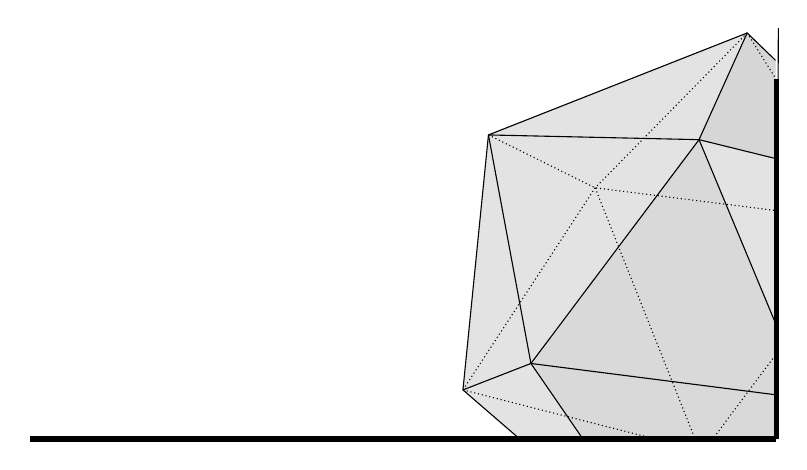
\begin{tikzpicture}[x=0.012cm,y=-0.012cm,line join=round]
\fill[gray!22] (497,139)--(771,31)--(801,60)--(801,460)--(529,460)--(470,409)--cycle;
\fill[gray!32] (771,31)--(720,144)--(801,164)--(801,60)--cycle;
\fill[gray!30] (542,381)--(720,144)--(800,336)--(800,460)--(595,458)--cycle;
\draw (497,139)--(771,31)--(801,60);
\draw (497,139)--(720,144)--(801,164);
\draw (771,31)--(720,144)--(800,336);
\draw (497,139)--(470,409)--(542,381)--(720,144);
\draw (497,139)--(542,381)--(595,458);
\draw (542,381)--(800,414);
\draw (470,409)--(529,460);
\draw[densely dotted] (497,139)--(610,195)--(801,219);
\draw[densely dotted] (771,31)--(610,195)--(470,409);
\draw[densely dotted] (610,195)--(715,459);
\draw[densely dotted] (470,409)--(662,458);
\draw[densely dotted] (736,459)--(801,372);
\draw[densely dotted] (771,31)--(801,79);
\draw (804,26)--(802,461);
\draw[line width=2pt] (802,80)--(802,461);
\draw[line width=2pt] (12,461)--(802,461);
\end{tikzpicture}}

\scanpage{2}
\unsure{Cohomologie} \deleted{\unsure{de} \illegible{1}} \unsure{galoisienne} \deleted{\illegible{1}}.
% archive sheet number: 1

\scanpage{3}
\deleted{\unsure{Corps de classes} \illegible{3}}

\unsure{Corps} de classes global \unsure{arithmétique|arithmétiques}

(énoncé des \unsure{théorèmes}...)

\deleted{\illegible{4}}
% archive sheet number: 2

\scanpage{4}
% source line 1: title
\uline{La Théorie \unsure{du} corps de classes}

% source lines 2-4
$K$ corps de \unsure{nbs|nbres} algébriques, ${\unsure{J|\mathscr{J}}}_K$ \unsure{groupe des} idèles, $U_K$ \deleted{\unsure{unités}} sous-groupe des idèles unités (à l'infini, \unsure{ils sont} $>0$ aux places réelles), ${\unsure{D|\mathscr{D}}}^a_K$ les diviseurs absolus, $D_K$ les diviseurs $(D^a_K\approx D_K\times Z_2^{r_1})$

% source line 4a: small interlinear addition
\inserted{Soit $\underline m$ un diviseur absolu, positif aux places finies (i.e. $\underline m_0$ est un idéal \uline{entier})}

% source lines 5-13
$D^{\underline m}_K$ les diviseurs premiers à $\underline m$ (ne dépend que de la partie finie $\underline m_0$ de l'idéal absolu $\underline m$), $P^{\underline m}_K\unsure{\subset|\in}D^{\underline m}_K$ \unsure{formé} des $(x)$ où $x\in K^*$ est $\equiv1\ (\underline m)$, i.e. $v_{\mathfrak p}(x\deleted{\unsure{+}}-1)\geq v_{\mathfrak p}(\underline m)$ aux places finies où $v_{\mathfrak p}(\underline m)>0$, et \deleted{$\unsure{x}$} $x\in K_{\mathfrak p}^{*+}$ aux places infinies où $v_{\mathfrak p}(\underline m)\neq0$. Les $x$ en question forment $K^{*(\underline m)}$. ${\unsure{\mathscr{P}|\mathfrak{P}|\mathcal{P}}}^{\underline m}_K=D^{\underline m}_K/P^{\underline m}_K$. (N.B. $K_{\deleted{\unsure{\mathfrak p}}}^{*\underline m}$ est aussi formé des quotients $x/y$, où $x$ et $y$ sont \uline{entiers} tels que $v_{\mathfrak p}(x-1)\geq v_{\mathfrak p}(\underline m)$ si $\mathfrak p$ est finie, et $x\in K_{\mathfrak p}^{*+}$ si $\mathfrak p$ est infinie et $v_{\mathfrak p}(\underline m)\neq0$. On a une suite exacte
\diagram{\[
\begin{tikzcd}[ampersand replacement=\&]
\&\&\&\&\text{classes d'idéaux}\\
0\arrow[r]\&N_K^{\underline m}\arrow[r]\&\mathscr{P}_K^{\underline m}\arrow[r]\&\mathscr{P}_K\arrow[r]\arrow[ur]\&0
\end{tikzcd}
\tag*{(1)}
\]}
où le noyau $N_K^{\underline m}$ se décrit ainsi
\[
0\longrightarrow Z_2^{S_\infty}/\operatorname{Im}E_K^{\underline m_0}\longrightarrow N_K^{\underline m}\longrightarrow(A_K/\underline m_0^{\deleted{\unsure{*}}})^*/\operatorname{Im}E_K\longrightarrow0
\tag*{(2)}
\]

% source lines 17-23
($A_K$, entiers de $K$, $E_K$ unités, $E_K^{\underline m_0}$ unités qui sont $\unsure{\approx|\equiv}1\ (\underline m_0)$), $S$ \unsure{ens} des places qui figurent dans $\underline m$, $S_\infty$ la partie infinie; N.B. Si $\underline m_0$ est grand, alors $E_K^{\underline m_0}$ est contenu dans n'importe quel sous-groupe d'indice fini \inserted{de $E_K$}, donc $\operatorname{Im}E_K^{\underline m_0}$ dans $Z_2^\infty$ est nul, donc $Z_2^\infty\unsure{\in|\subset}N_K^{\underline m}$ !). Si $\underline m$ est fini, i.e. $S_\infty=\varnothing$, alors on a la suite exacte
\[
0\longrightarrow(A_K/\underline m_0)^*/\operatorname{Im}E_K\longrightarrow\mathscr{P}_K^{\underline m}\longrightarrow\mathscr{P}_K\longrightarrow0.
\]

% source lines 24-25
Soit $C_K=J_K/K^*$, $U_K^{\deleted{\unsure{S}}\underline m}=\displaystyle\prod_{\mathfrak p\in\complement S}K_{\mathfrak p}^*\times\prod_{\mathfrak p\in S_0}(\deleted{\unsure{K_{\mathfrak p}}}1+\mathfrak p^{v_{\mathfrak p}(\underline m)})\times\prod_{\mathfrak p\in S_\infty}K_{\mathfrak p}^{*+}$, i.e. \unsure{c'est} l'\unsure{ens} des \uline{idèles} qui sont $\equiv1\ (\underline m)$.

% source lines 26-29
Alors $U_K^{\unsure{\complement S|\underline m}}$ est un voisinage \unsure{ouvert} de $0$ dans $J_K$ (et si $\underline m$ varie, on obtient un \unsure{syst.} fondamental de tels \unsure{sous-gps}), et \deleted{$\unsure{C_K/\operatorname{Im}U_K^{\underline m}}$} on a
\[
C_K/\operatorname{Im}U_K^{\underline m}\approx\mathscr{P}_K^{\underline m}.
\]
% archive sheet number: 3

\scanpage{5}
% source lines 1-2
Par suite, on a
\[
\varprojlim_{\underline m}{\unsure{\mathscr{P}|\mathfrak{P}|\mathcal{P}}}_K^{(m)}=C_K/\substack{\text{composante}\\\text{de l'unité}}\,D_K=C'_K.
\]

% source lines 3-9
Si $L$ est une extension \deleted{galoisienne} \inserted{finie} de $K$, on a
\[
\mathscr{P}_K^{\underline m}/N_{L/K}\mathscr{P}_L^{\underline m'}\approx C_K/N_{L/K}C_L
\]
pourvu que $N_{L/K}{\unsure{J|\mathscr{J}}}_L\supset U^{\underline m}$ (ce qui est vrai si $\underline m$ est assez grand, --- il suffit de le prendre grand \unsure{uniquement} aux \unsure{premiers sur} les places \uline{ramifiées} de $L$) et $\underline m$ étant \unsure{choisi ainsi}, $\underline m'$ (idéal absolu de $L$) est pris assez grand pour que $N_{L/K}L^{*\underline m'}\subset K^{*\underline m}$.

% source lines 10-15
\inserted{Supposons $L$ galoisienne.} On a un hom canonique (si $S$ désigne l'ens des places \inserted{\unsure{non}} ramifiées finies de $L$).
\[
{\unsure{D|\mathscr{D}}}^{\deleted{\unsure{\underline m}}S_0}\longrightarrow G(L/K)
\]
par la condition que si $\mathfrak p\notin S_0$, $\mathfrak p\unsure{-|\mapsto}(\mathfrak p,L/K)$ (substitution de Frobenius). Le noyau contient \deleted{\unsure{les}} $N_{L/K}D_{L\deleted{\unsure{K}}}^{S'_0}$ (trivial). La théorie du corps de classes

% source lines 16-20, circled a
\textcircled{a} affirme qu'on peut trouver $\underline m$ (\unsure{formé|premier} avec $S$) tel que \deleted{\unsure{tout} $(x)$} $P_K^{\underline m}$ est dans le noyau; elle implique
\diagram{\begin{tikzcd}[ampersand replacement=\&]
\text{qu'on a un hom. canonique}\&\mathscr{P}_K^{\underline m}\arrow[r]\arrow[d,phantom,"\wr" description]\&G(L/K)\\
\text{d'où un hom canonique}\&C_K/\operatorname{Im}U_K^{\underline m}\arrow[r]\&G(L/K)
\end{tikzcd}}

(et en fait un hom.
\diagram{\begin{tikzcd}[ampersand replacement=\&]
\mathscr{P}_K^{\underline m}/\unsure{N_{L/K}|\deleted{N_{L/K}}}\mathscr{P}_{\unsure{K|L}}^{m'}\arrow[r]\arrow[d,phantom,"\wr" description]\&G(L/K)\\
C_K/N_{L/K}C_L\arrow[ur]\&
\end{tikzcd}}
)

% source lines 21-26
% slanted
\margin{\uline{hom. de réciprocité}}
\unsure{Cela|Ceci} permet donc de définir, pour \deleted{\unsure{tout}} \uline{idèle} $\underline a$, \unsure{les éléments|l'élément} $(\underline a,L/K)\in G(L/K)$, \deleted{et} $(\underline a,L/K)_{\mathfrak p}=(\underline a_{\mathfrak p},L/K)$ (``\unsure{Normenrestsymbol}'' de Hilbert), c'est un hom. continu, défini par les conditions : $(\underline a_{\mathfrak p},L/K)=(\mathfrak p,L/K)$ si $\mathfrak p$ fini non ramifié \inserted{et} $v_{\mathfrak p}(a_{\mathfrak p})=1$, et $(\unsure{x},L/K)=\unsure{1|0}$ si \deleted{$\unsure{a}=$} $x\in K^{*\underline m}$ ($\underline m$ grand). De plus

% source lines 27-28, circled b
\textcircled{b} L'hom $D_K^{S_0}\longrightarrow G(L/K)$ est surjectif, (et même on a le ``\uline{th. de la progression arithmétique}'') et

% source lines 29-30, circled c
\textcircled{c} Son noyau est \uline{exactement} $P_K^{\underline m}N_{L/K}{\unsure{P|D}}_L^{m'}$, i.e. on a un \uline{isomorphisme}
\[
\mathscr{P}_K^{\underline m}/N_{L/K}\mathscr{P}_L^{m'}=C_K/N_{L/K}C_L\longrightarrow G(L/K).
\]
% archive sheet number: 4

\scanpage{6}
% source lines 1-2
Soit $K$ un corps de nombres fini sur $\mathbb Q$.

Pour toute place $\mathfrak p$ de $K$ (finie ou infinie), on considère
\[
\left\{\begin{aligned}
&K_{\mathfrak p}\ \text{corps local de }\mathfrak p\quad(\approx\mathbb R\text{ ou }\mathbb C\text{ si }\mathfrak p\text{ est infini})\\
&U_{\mathfrak p}\ \text{ens des éléments de }{\unsure{U|K}}_{\mathfrak p}\text{ tels que }|a|_{\mathfrak p}=1\quad(\text{unités de }\mathfrak p)\ (\pm1\text{ ou }\mathbb T\text{ à l'infini})\\
&W_{\mathfrak p}=K_{\mathfrak p}^*/U_{\mathfrak p}\quad\text{groupe des valeurs}\quad(\mathbb Z:\text{\unsure{distance} finie},\mathbb R^{*+}\text{ à l'infini})
\end{aligned}\right.
\]
\margin{\figure{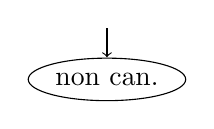
\begin{tikzpicture}\draw[->] (0,.65)--(0,.28);\draw (0,0) ellipse (1cm and .27cm);\node at (0,0) {\unsure{non can.}};\end{tikzpicture}}}

% source lines 6-8
$\bigl(\ \unsure{J|\mathscr{J}}(K)\subset\prod K_{\mathfrak p}^*$, défini comme l'image inverse de $\coprod W_{\mathfrak p}$ par $\prod K_{\mathfrak p}\longrightarrow\prod W_{\mathfrak p}$. Topologie
\inserted{(idèles)}

$\bigl(\ {\unsure{D|\mathscr{D}}}_{\mathrm{abs}}(K)=\underset{\mathfrak p}{\coprod^{\deleted{\unsure{\prod}}}}W_{\mathfrak p}$

$\bigl(\ V(K)$ (idèles unités) $=\prod U_{\mathfrak p}$, donc on a une suite exacte
\[
0\longrightarrow V(K)\longrightarrow J(K)\longrightarrow D_{\mathrm{abs}}(K)\longrightarrow0.
\]

% source lines 9-12
\deleted{\unsure{P(K)=}}\inserted{($K^*$ idèles principaux, \uline{discret} \uline{dans} $J(K)$)}

$\bigl(\ C(K)=J(K)/\deleted{\unsure{P}}K^*$ (compte tenu de l'application diagonale $K^*\longrightarrow J(K)$)
\[
0\longrightarrow K^*\longrightarrow J(K)\longrightarrow C(K)\longrightarrow0
\]

% source lines 13-15
$\bigl(\ \unsure{\mu|U}(K)=$ racines de l'unité de $K=$ torsion de
\diagram{\begin{tikzcd}[ampersand replacement=\&]K^*\unsure{\infty|\deleted{=}}\arrow[d]\\\text{\unsure{th. particulier}}\end{tikzcd}}
\margin{$P\cap V=$ unités absolues de $K$}


$\bigl(\ {\unsure{\mathscr{P}|\mathfrak{P}|\mathcal{P}}}_{\mathrm{abs}}(K)=D_{\mathrm{abs}}(K)/\operatorname{Im}K^*$ d'où

\deleted{$\unsure{E(K)}=$}
\[
0\longrightarrow\mu(K)\longrightarrow K^*\longrightarrow D_{\mathrm{abs}}(K)\longrightarrow\mathscr{P}_{\mathrm{abs}}(K)\longrightarrow0
\]

% source lines 16-18
$\bigl(\ J(K)\longrightarrow\mathbb R^{*+}$ l'hom norme déduit de $D_{\mathrm{abs}}(K)\longrightarrow\mathbb R^{*+}$,

$\bigl(\ J_0(K)$ et $D_{\mathrm{abs},0}(K)$ les idèles et diviseurs abs. de norme $1$.

On a $K^*\unsure{\in|\subset}J_0(K)$ d'où
\[
\left\{\begin{aligned}
&\mathscr{P}_{\mathrm{abs}}(K)\longrightarrow\mathbb R^{*+}\quad\text{et }\mathscr{P}_{\mathrm{abs},0}(K)\\
&C(K)\longrightarrow\mathbb R^{*+}\quad\text{et }C_0(K)
\end{aligned}\right.
\]

% source: large lower diagram
\diagram{\begin{tikzcd}[ampersand replacement=\&,column sep=small,row sep=large]
\&\&V(K)\arrow[dr,"\text{diviseurs abs. principaux}" description]\arrow[drr,"D_{\mathrm{abs},0}(K)",bend left=8]\arrow[drrr,"D_{\mathrm{abs}}(K)",bend left=13]\&\&\&\\
0\arrow[r]\&\mu(K)\arrow[ur]\arrow[dr]\&\&K^*V(K)\arrow[r,"\deleted{\unsure{\text{classes absolues}}}","\mathscr{P}_{\mathrm{abs},0}(K)"']\&J_0(K)\arrow[r,"\mathbb R^{*+}"']\&J(K)\\
\&\&K^*\arrow[ur,"\unsure{\text{ramification}}" description]\arrow[urr,"C_0(K)"',bend right=8]\arrow[urrr,"C(K)"',bend right=20]\&\&\&
\end{tikzcd}}

% source lines 19-22
\uline{Th. de Dirichlet} $C_0(K)$ est compact

La démonstration se fait par Minkowski.

Comme $K^*V(K)/K^*$ est comp., le th. \unsure{équivaut} au fait que le groupe $D_{\mathrm{abs},0}(K)/\operatorname{Im}K^*$ des classes
% archive sheet number: 5

\scanpage{7}
% source lines 1-2, continuation of scan 6
de diviseurs absolus \inserted{(de \deleted{norme} valeur absolue $1$)} est compact. Or on a
\[
{\unsure{D|\mathscr{D}}}_{\mathrm{abs}}(K)\simeq D(K)\times D_\infty(K)
\]

% source lines 3-5
\deleted{où $D(K)$ est le \unsure{gr.}}
\[
\left\{\begin{aligned}
&D(K)\quad\text{groupe des diviseurs usuels de }K\\
&D_\infty(K)=\coprod_{\mathfrak p\text{ à l'infini}}W_{\mathfrak p}\quad\text{groupe des diviseurs à l'infini}
\end{aligned}\right.
\]

% source lines 6-8
On \deleted{$\unsure{K}$} écrira
\[
0\longrightarrow D_{\infty,0}(K)\longrightarrow D_{\mathrm{abs},0}(K)\longrightarrow D(K)\longrightarrow0
\]
et on considère dans $D_{\mathrm{abs},0}(K)$ l'image de $K^*$, soit $P\simeq K^*/\unsure{\mu|U}(K)$ \deleted{\unsure{des}} diviseurs absolus principaux.

On a alors
\[
0\longrightarrow D_{\infty,0}(K)/E_0(K)\longrightarrow{\unsure{\mathscr{P}|\mathfrak{P}|\mathcal{P}}}_{\mathrm{abs},0}(K)\longrightarrow\mathscr{P}(K)\longrightarrow0.
\]

% source lines 10-14
où on pose
\[
\begin{aligned}
\bigl(\quad&\mathscr{P}(K)=D(K)/\operatorname{Im}K^*=D_{\mathrm{abs}}(K)/P+D_\infty(K)\\
\bigl(\quad&E_0(K)\simeq P\cap D_\infty^{\deleted{\unsure{0}}}(K)\simeq(P+D_\infty(K))/P\simeq\deleted{\unsure{E(K)}}E(K)/\mu(K),\ \text{\unsure{où}}.
\end{aligned}
\]
$\bigl(\ E(K)\simeq$ unités de $K$ i.e. \unsure{élmts|éléments|élts} de $K^*$ dont l'image dans $D_{\mathrm{abs}}(K)$ est dans $D_\infty(K)$.

% source lines 15-16
\deleted{\unsure{D'autre part, le}} Ceci dit, le th. de \deleted{Minkowski} \inserted{Dirichlet} \unsure{équivaut} à \unsure{l'ens|l'un} des deux corollaires

% source lines 17-20
\uline{Cor. 1} $\mathscr{P}(K)$ est fini

\uline{Cor. 2} $E_0(K)$ est de rang $r_1+r_2-1$

(i.e. la dimension de $D_{\infty,0}(K)$). D'où

\uline{Cor. 3} $\mathscr{P}_{\mathrm{abs},0}(K)$ est une extension de $\mathscr{P}(K)$, \unsure{qui est} un \unsure{grp|gpe} fini, par un tore de dim. $r_1+r_2-1$.
% archive sheet number: 6

\scanpage{8}
% source lines 1-4
On s'intéresse aux sous-groupes \inserted{ouverts} de $C(K)$ \deleted{\unsure{contenant la partie connexe}}, i.e. aux sous-groupes \inserted{ouverts} de $\unsure{J|\mathscr{J}}(K)$ contenant $K^*$. Un tel sous-groupe $M$ contient \unsure{aussi} $J_\infty^{\mathrm{conn}}\deleted{\unsure{\subset}}=J^{\mathrm{conn}}$, \deleted{et} un sous-groupe \deleted{$\unsure{H_{\underline m}V_\infty}$} $V_{\underline m}$ [où

% source lines 5-8
\diagram{\begin{tikzcd}[ampersand replacement=\&,column sep=0.5em,row sep=small]
\bigl(\quad V_{\underline m}=\prod_{\substack{\unsure{\mathfrak p\nmid\underline m|\mathfrak p\mid\underline m}\\\mathfrak p\text{ fini}}}\&V_{\underline m,\mathfrak p}\arrow[dr]\&\subset\deleted{\unsure{C_a}}\subset{\unsure{D|\mathscr{D}}}_{\mathrm{abs}}\\
\&\&\begin{gathered}\underline m\text{-unités;}\\\text{à distance infinie, cela est }J_\infty^{\mathrm{conn}};\\\text{si }\mathfrak p\nmid\underline m,\text{ cela est }V_{\mathfrak p}\end{gathered}
\end{tikzcd}}
\[
\begin{aligned}
\bigl(\quad&J_{\underline m}=J\cap\prod_{\mathfrak p\nmid\underline m}K_{\mathfrak p}\\
\bigl(\quad&D_{\underline m}=J_{\underline m}/V_{\underline m}\cap J_{\underline m}\simeq\coprod_{\mathfrak p\nmid\underline m}\deleted{\unsure{V}}W_{\mathfrak p}=\mathbb Z^{\pi(\underline m)}
\end{aligned}
\]
($\underline m$ est un diviseur absolu contenant les places à l'$\infty$)
\margin{$\pi(\underline m)$ ens des diviseurs premiers $\nmid\underline m$}
(diviseurs premiers à $\underline m$)
]

% source lines 9-11: cancelled block
\deleted{et un sous-groupe $\displaystyle\prod_{\substack{\mathfrak p\text{ fini}\\\mathfrak p\mid\underline m}}A_{\mathfrak p}\unsure{\simeq|=}A'$ où pour tout $\mathfrak p$ fini, $\mathfrak p\mid\underline m$, $A_{\mathfrak p}$ est un voisinage de $1$ dans $K_{\mathfrak p}$.}

% source lines 12-18
Donc $M\supset\deleted{\unsure{H_{\underline m}=(V_{\underline m}\times\prod_{\mathfrak p\mid\underline m,\ \mathfrak p\text{ fini}}A_{\mathfrak p}\times J_\infty^{\mathrm{conn}})}}V_{\underline m}K^*$, et réciproquement, si \inserted{\unsure{$M$ contient un $H_{\underline m}$}}, ....

Je dis qu'on a $\deleted{\unsure{H_{\underline m}}}K^*V_{\underline m}+J_{\underline m}=J$, ce qui \unsure{résulte|résultera} du fait que, \deleted{$\unsure{V_{\underline m}\in A'\times J_\infty^{\mathrm{conn}}}$} \inserted{$V_{\underline m}\cap\displaystyle\prod_{\mathfrak p\mid\underline m}K_{\mathfrak p}$} est un voisinage de $1$ dans $\deleted{\unsure{J}}\displaystyle\prod_{\mathfrak p\mid\underline m}K_{\mathfrak p}$, il existe pour tout $\vec x_{\unsure{\mathfrak p|\underline m}}\in\displaystyle\prod_{\mathfrak p\mid\underline m}K_{\mathfrak p}$ un $a\in K^*$ tel que $a_{\mathfrak p}^{-1}\vec x\in V_{\underline m}\deleted{\unsure{\times V_\infty}}$; Ainsi,

% source lines 19-21
On aura
\[
J/K^*V_{\underline m}\simeq J_{\underline m}/K^*V_{\underline m}\cap J_{\underline m}
\]
\deleted{\unsure{on}} et \deleted{\unsure{comme}} d'autre part, comme $H_{\underline m}\supset V_{\underline m}\cap J_{\underline m}$, \deleted{\unsure{on}} on a
\[
J/H_{\underline m}\simeq D_{\underline m}(K)/P_{\underline m}(K)
\]

% source lines 22-24 and lower margin
où $P_{\underline m}(K)=$ \unsure{ens|\deleted{les}} des diviseurs \deleted{\unsure{principaux}} \inserted{premiers à $\underline m$} de la forme $\operatorname{div}(\vec y)$, i.e. $\vec y=a\cdot\vec x\deleted{\unsure{\vec x_{\underline m}\times\vec x_\infty}}$ avec

\deleted{$a\in K^*,\quad\vec x'_{\underline m}\times\vec x''_{\underline m}\times\vec x_\infty\in(J_{\underline m}\cap V_{\underline m})\times\unsure{\vec x'_\infty}$}

$a\in K^*$, $\vec x\in V_{\underline m}$, $\deleted{\unsure{\operatorname{div}(\vec y)\in D_{\underline m}}}\quad y_{\mathfrak p}=1\text{ si }\mathfrak p\mid\underline m$.
% slanted
\margin{diviseurs \unsure{non} absolus}
% archive sheet number: 7

\scanpage{9}
% source lines 1-4
Or on a $\operatorname{div}(\vec y)\equiv\operatorname{div}(a)$ (car $\operatorname{div}(\vec x)=\unsure{1|0}$) et il faut donc prendre les $\operatorname{div}(a)$, où $a\in K^*$ est tel que $a_{\mathfrak p}\in V_{\mathfrak p,\underline m}$ si $\mathfrak p\mid\underline m$, --- \unsure{ce qui s'écrit}
\[
a\equiv1\ (\underline m).
\]

On a par suite

\deleted{$\unsure{C\simeq J/V_{\underline m}K^*}$}
\[
C_{\underline m}(K)=C(K)/H_{\underline m}(K)\simeq\unsure{J|\mathscr{J}}(K)/V_{\underline m}(K)K^*\simeq{\unsure{D|\mathscr{D}}}_{\underline m}(K)/P_{\underline m}(K)
\]

% source lines 7-10
avec

$P_{\underline m}(K)=$ \unsure{classes de diviseurs} de la forme $(a)$, avec $a\equiv1\ (\underline m)$ (ce qui \deleted{signifie} \inserted{implique} que $a$ est \uline{positif} aux places à l'infini réelles).

$H_{\underline m}(K)=V_{\underline m}(K)K^*/K^*$. On a aussi

% source: exact sequence and its two annotations
\diagram{\begin{tikzcd}[ampersand replacement=\&,column sep=small]
0\arrow[r]\&\substack{\text{ss-groupe de }\deleted{\unsure{E(K)^*}}\inserted{E(K)}\text{ formé}\\\text{des éléments qui sont}\\\equiv1\ (\underline m)\\\text{[ce qui implique}\\\text{qu'ils sont }\geq0\text{ aux places}\\\text{réelles]}}\arrow[r]\&K^*\arrow[r]\&\deleted{\unsure{P}}\underbrace{D_{\underline m}(K)\times\displaystyle\prod_{\substack{\deleted{\unsure{\mathfrak p\text{ fini}}}\\\mathfrak p\mid\underline m}}}\underbrace{K_{\mathfrak p}/V_{\mathfrak p,\underline m}}_{\substack{\mathbb Z/2\text{ aux places}\\\text{réelles, }0\text{ aux}\\\text{places complexes,}\\\text{sinon une extension}\\\text{de }\mathbb Z\text{ par un groupe}\\\deleted{\text{\unsure{d'ordre}}\ \unsure{Z_{\mathfrak p}}}\ ......}}\arrow[r]\&C_{\underline m}(K)\arrow[r]\&0
\end{tikzcd}}

% source lines 11-15
Soit $x\in K_{\mathfrak p}$, où $\mathfrak p$ est une place quelconque.

Alors $x$ définit un \unsure{élmt|èlmt|élément} de $J(K)$, donc de $C(K)$ donc de $C_{\underline m}(K)$, donc de $D_{\underline m}(K)/P_{\underline m}(K)$.

Pour le calculer, \deleted{\unsure{on sait que}} \deleted{\unsure{on fait la chose}} \unsure{il vient} $\operatorname{div}(x)\bmod P_{\underline m}(K)$ si $\mathfrak p\nmid\underline m$. \uline{Si} $\mathfrak p\mid\underline m$, $\longrightarrow$
% archive sheet number: 8

\scanpage{10}
% source lines 1-4, continuation
\unsure{je} \unsure{considère|considérer} un $a\in K^*$ tel que
\[
\left\{\begin{aligned}
a&\equiv1\ (\underline m)\quad\text{aux places }\deleted{\unsure{\mathfrak p}}\ \unsure{\mathfrak q|v}\mid\underline m,\ \mathfrak q\neq\mathfrak p\\
a&\equiv x\quad\underline m\quad\text{en }\mathfrak p
\end{aligned}\right.
\]
[\deleted{\unsure{la définition}} Si $a'$ en est un autre, alors $aa'^{-1}\deleted{\unsure{\in K}}\equiv1\ (\underline m)$]

On prend alors $\operatorname{div}_{\complement\underline m}(a)\bmod P_{\underline m}(K)$.

% source lines 5-12
\uline{\unsure{Ènoncé|Énoncé} des \unsure{théorémes|théorèmes} de Artin--Takagi}. Soit $L$ une extension \unsure{galoisienne} \inserted{finie} de $K$. \deleted{\unsure{Pour de}} Soit $S$ l'ens des places de $K$ où $L$ est ramifié. Pour $\mathfrak p\in\complement S$, on définit $\sigma(\unsure{\mathfrak P|\mathscr P})\in\operatorname{Gal}(L/K)=G$ \inserted{(substitution de Frobenius)} dans le groupe de décomposition d'un $\mathfrak P$ au-dessus de $\mathfrak p$ (si on change $\unsure{\mathfrak p|\mathfrak P}$, $\sigma(\mathfrak P)$ ne change que par un aut. intérieur), et définit donc un $\unsure{=}$ élément de $G/G'$. \deleted{Alors} \inserted{On} prolonge par linéarité en un hom.
\[
{\unsure{D|\mathscr{D}}}_{\underline m}(K)\longrightarrow G/G'\qquad(\text{hom. de réciprocité})
\]

% source lines 13-17, circled 1 degree
\textcircled{$1^\circ$} \uline{\uuline{On peut trouver un module}} $\underline m$, de support $S$, t.q. l'hom de réciprocité s'annule sur $P_{\underline m}(K)$.

On peut donc le considérer comme un hom
\[
C_{\underline m}(K)\longrightarrow G/G',
\]
\inserted{donc $C(K)\longrightarrow G/G'$}
(cet dernier ne dépend plus du choix de $\underline m$]
\margin{[\unsure{n'a} de sens que dans $G/G'$ !]}

% source lines 18-23, circled 2 degree
\textcircled{$2^\circ$} \uline{Cet hom. est surjectif} [de façon plus précise, pour $\forall$ classe d'\unsure{élmts|élts} de $G$, il existe une \uline{infinité} de places $\mathfrak p$ pour \unsure{lesquels|lesquelles} $\sigma(\mathfrak p)$ soit dans cette classe]. Ainsi, $G/G'$ est un \uline{quotient} de $C_{\underline m}(K)$

% source line 24, continuing on scan 11
\textcircled{$3^\circ$} Le \uline{noyau de l'hom de réciprocité} est
% archive sheet number: 9

\scanpage{11}
% source lines 1-3, continuation of 3 degree
\uline{exactement} \inserted{(contient trivialement)} \unsure{l'im.} \deleted{des classes} $N_{L/K}C(L)$. En d'autres termes le noyau de ${\unsure{D|\mathscr D}}_{\underline m}(K)\unsure{-|\longrightarrow}G/G'$ est \uline{exactement} \inserted{(contient trivialement)} $P_{\underline m}(K).N_{L/K}(D_{\underline m'}(L))\deleted{\unsure{\}}}$.

% source lines 4-6
Cela montre déjà que les extensions \uline{abéliennes} \inserted{\uline{finies}} de $K^*$ correspondent à \deleted{\unsure{des}} \uline{certains} sous-groupes ouverts de $C(K)$. Il y a de plus un

% source lines 7-15, circled 4 degree
\textcircled{$4^\circ$} \uline{Théorème d'existence} : \deleted{Pour} Tout sous-groupe ouvert de $C(K)$ correspond à une extension abélienne, i.e. Pour \unsure{tout|$\forall$} module $\underline m$, il existe une extension abélienne $L$ de $K$ \inserted{admettant le module $\underline m$ et} telle que
\[
N_{L/K}(D_{\underline m}(L))\subset\deleted{\unsure{D_{\underline m}}}P_{\underline m}(K).
\]
[ou aussi : pour $\forall$ ss-groupe ouvert $U$ de $C(K)$, existe une extension abélienne $L$ de $K$, t.q. $N_{L/K}C(L)=U$].

% source lines 16-21
N.B. \unsure{L'essentiel} de ces assertions ne concerne que les extensions abéliennes \deleted{\unsure{les autres}} (en fait, la sous-extension abélienne maximale $L_{\unsure{a|0|o}}$ de $K$ dans $L$). Les assertions faites équivalent \unsure{à|aux} ces assertions pour $L$ abélien, plus le fait que $N_{L/K}C(L)=N_{L_a/K}C(L_a)$
% archive sheet number: 10

\scanpage{12}
% source lines 1-4
La grande conséquence de $\uline{1^\circ}$ est la possibilité de définir $C(K)\longrightarrow G/G'$, i.e. essentiellement de savoir définir des \unsure{hom|homs}
\[
\boxed{K_{\mathfrak p}^*\longrightarrow G/G'}
\]
(notation $\left(\dfrac{x,L/K}{\mathfrak p}\right)$) de telle façon qu'on ait
\[
\boxed{\prod_{\mathfrak p}\left(\frac{x,L/K}{\mathfrak p}\right)=1\qquad\text{si }x\in K^*}
\]

% source lines 7-10
[si $\mathfrak p$ est non ramifiée, le symbole \unsure{de|d'} \deleted{Artin} \deleted{est} \unsure{canonique} étant défini par l'hom de \unsure{Frobénius|Frobènius|Frobênius}]. Le lien avec la \uline{théorie des corps de classes \unsure{local|locale}} est le suivant :

% source lines 11-15
On a pour tout $\mathfrak p$, \unsure{des hom naturels|des homs naturels|un hom naturel}
\diagram{\begin{tikzcd}[ampersand replacement=\&]
A(K_{\mathfrak p})\arrow[r,"\text{surj.}"]\&
\begin{gathered}\text{groupe de décomposition }G_{\mathfrak p}^{d}\\\text{de }G\text{ relatif à }\mathfrak p\end{gathered}
\end{tikzcd}}
(on suppose $L/K$ abélien pour simplifier) où $A(K_{\mathfrak p})$ désigne le groupe de \unsure{galois|Galois} de l'extension abélienne maximale de $K_{\mathfrak p}$. D'autre part d'après la théorie du corps de classes \unsure{local|locale|locales} on a un isomorphisme canonique
% archive sheet number: 11

\scanpage{13}
% source lines 1-3
\[
A(K_{\mathfrak p})\simeq K_{\mathfrak p}^*
\]
de sorte qu'on a des épimorphismes
\[
{\unsure{\varphi|\phi}}_{\mathfrak p}:K_{\mathfrak p}^*\longrightarrow G_{\mathfrak p}^{d}
\]

% source lines 4-5, circled 5 degree
\textcircled{$5^\circ$} \uline{Ces applications sont précisément les hom. de réciprocité, \unsure{donnés|données} par les symboles de \deleted{\unsure{Art|Artin}} \inserted{\unsure{restes}} \unsure{normiques}.}

% source lines 6-12
Comme les deux applications coïncident manifestement aux places non ramifiées, l'assertion (5) équivaut au fait que ces homs $\varphi$ \inserted{\unsure{continus|continu}} proviennent bien d'un hom unique $C(K)\longrightarrow G_{\mathfrak p}^{d}$, i.e. \unsure{ils|il} \uline{signifient} \uline{essentiellement} que l'on a la formule
\[
\boxed{\prod_{\mathfrak p}\varphi_{\mathfrak p}(x_{\mathfrak p})=1\qquad\text{si }x\in K^*}
\]

% source lines 14-16
(Formule qui \deleted{\unsure{est loin d'être}} équivaut à la partie difficile de la théorie \unsure{actuelle} des corps de classes pour les corps de \unsure{nbs|nbres}).
% archive sheet number: 12

\scanpage{15}
% upper detached cancelled object and arrow
\diagram{\begin{tikzcd}[ampersand replacement=\&]
\deleted{\unsure{\mathscr W|\mathfrak W}}_G\arrow[r]\&{}
\end{tikzcd}}
% upper left diagram; unheaded strokes retained as dashes
\diagram{\begin{tikzcd}[ampersand replacement=\&,column sep=small,row sep=small]
\&0\arrow[dr]\&\&\&\&\\
\&G(C)\arrow[r]\arrow[dr]\&{\unsure{\mathscr U|\mathfrak U|U}}_G(k)\arrow[dr]\&\&{}\&\\
0\arrow[rr,dash]\&\&G(K)\arrow[r]\&{\unsure{\mathscr W|\mathfrak W|W}}_G(k)\arrow[r]\arrow[dr]\&{\unsure{\mathscr J|\mathfrak J|\mathcal J|J}}_G(k)\arrow[r]\arrow[ur,dash]\arrow[dr]\&0\\
\&\&\&\&{\unsure{D|\mathscr D}}_G(k)\arrow[r,dash]\arrow[dr]\&J_{G\unsure{/|,}C}\arrow[dr,squiggly]\\
\&\&\&\&\&0\&\operatorname{Hom}(\mathbb G_m,G)
\end{tikzcd}}

% upper right block; the upper Hom and upward arrow are in pencil
\diagram{\begin{tikzcd}[ampersand replacement=\&]
\operatorname{Hom}(G_m,G)\\
H^{\unsure{\mu|1|u}}(C,G)=J_{G/\underline C}(k)\arrow[u]
\end{tikzcd}}
\margin{le noyau est formé des \unsure{classes} sur $C$ qui proviennent de $\operatorname{Ext}^1(J_C,G)$}
% pencil enclosure around the right block
\figure{\begin{tikzpicture}[scale=.35]
\draw[gray] (6,5) .. controls (1,4.7) and (-1,4.3) .. (0,1.4)
.. controls (.5,.5) and (3,.7) .. (4,.2)
.. controls (5,-.4) and (4.5,-2.3) .. (7,-3);
\end{tikzpicture}}

% line below upper diagram
$G(C)\qquad(=G(k)\text{ si }G\text{ est linéaire})$

% middle diagram; arrowheads only where visible
\diagram{\begin{tikzcd}[ampersand replacement=\&,column sep=small,row sep=small]
\&0\arrow[dr]\&\&\&\&\\
\&k^*\arrow[r,dash]\arrow[dr]\&\mathscr U(k)\arrow[dr,dash]\&\&\&\\
0\arrow[rr,dash]\&\&K^*\arrow[r,dash]\&\mathscr W(k)\arrow[r,dash]\arrow[dr]\&J(k)\arrow[r,dash]\arrow[dr]\&0\\
\&\&\&\&D(k)\arrow[r]\arrow[dr]\&J_C(k)\arrow[dr]\\
\&\&\&\&\&0\&\operatorname{Hom}(\mathbb G_m,\mathbb G_m)=\mathbb Z
\end{tikzcd}}
\margin{$H^1(C,\mathbb G_m)=J_C(k)$}
\[
\mathbb G_m(C)=k^*
\]

% bottom pairing block
\[
\mathscr W_G(k)\times\mathscr W(k)\longrightarrow G(k)\qquad\text{grâce aux symboles locaux}
\]
\[
\left\{\begin{aligned}
\mathscr U_G(k)\times\mathscr U(k)&\longrightarrow0&&\text{théorie locale des symboles locaux}\\
G(K)\times K^*&\longrightarrow0&&\text{théorie globale (Rosenlicht)}
\end{aligned}\right.
\]
\deleted{\unsure{d'où|si} $\unsure{D_G(k)}$}
\[
\mathscr W_G(k)^0\times k^*\longrightarrow0\qquad\text{vu définition de }\mathscr W_G(k)^0
\]
\[
G(C)\times\mathscr W(k)^0
\]
% archive sheet number: 14

\scanpage{16}
% top two pairings and their right-hand explanations
\[
G(K)\times\unsure{J|\mathscr J}(k)\longrightarrow G(k)\qquad
\text{(définition de }J\text{ comme \unsure{albanese|albanaise} \unsure{généralisée|généralisé})}
\]
\[
J_G(k)\times K^*\longrightarrow G(k)\qquad\text{application spéciale}
\]

% next two pairings
\[
{\unsure{\mathscr U|\mathfrak U|U}}_G(k)\times\unsure{D|\mathscr D}(k)\longrightarrow G(k)
\qquad\text{\inserted{\unsure{trivial}} à l'aide des augmentations}
\]
\[
D_G(k)\times\mathscr U(k)\unsure{-|\longrightarrow}G(k)\qquad\text{théorie des symboles locaux}
\]

% central pairing and provenance
\[
J_{G,C}\times k^*\longrightarrow G(k)
\]
Provient de $J_{G,C}\longrightarrow\operatorname{Hom}_{\text{\unsure{k-gr|k-g}}}(\mathbb G_m,G)$, noyau $J_{G,C}^0$

\[
G(C)\times J_C(k)\longrightarrow G(k)
\]
\margin{provient de l'application $\deleted{\unsure{\varphi}}\operatorname{Hom}(C,G)\longrightarrow\operatorname{Hom}(J_C,G)$ [définition de $J_C$] si $G$ est linéaire, alors \deleted{est \uline{nulle}} $G(C)\simeq G(k)$ \unsure{cette} application provient de l'augmentation $J_C(k)\unsure{-|\longrightarrow}\mathbb Z$}

% lower paragraph
Soit $J'_C(k)\subset J_C^0(k)$ l'intersection des noyaux des hom de \unsure{grps|groupes} algébriques : $J_C^0\unsure{-|\longrightarrow}G$ (c'est donc $J_C^0(k)$ si $G$ est linéaire)

% boxed formula, with the two underbrace identifications
\[
\boxed{\xi\in\operatorname{Ext}^1\left(
\underbrace{J_{G,C}^0(k)}_{\substack{\Vert\\\operatorname{Ext}^1(J_C^{\unsure{0|\bullet}},{\unsure{G|\mathbb G}}_{\deleted{\unsure{m}}})}},
\underbrace{J'_C(k)}_{\substack{\unsure{\cap|\uparrow}\\\operatorname{Ext}^1(J_C^0,\unsure{\mathbb G_m|G_m})}};
G(k)\right)}
\]
\margin{accouplement de Lang.}
% archive sheet number: 15
